 %GPL V3 by Mathias Hablützel, feel free to improve this template
 \documentclass[a4paper,10pt]{article}
 
 % Use UTF8 since the laptop is configured so and use ngerman for word breaking.
 % If you encounter an encoding problem, remove the line with utf8.
 \usepackage[utf8]{inputenc}
 \usepackage[ngerman]{babel}
 \usepackage[pdftex]{graphicx}
 
 % TikZ für schöne Grafiken und so.
 \usepackage{tikz}
 \usetikzlibrary{positioning,calc,fadings,decorations.pathreplacing,arrows}
 \usepackage{pgfplots}

% \usepackage{hyperref}
 \usepackage{colortbl}
 \usepackage{tabularx}
 \usepackage{color}
 \usepackage{amsfonts}
 \usepackage{amsmath}
 \usepackage{listings}
 \usepackage{multirow}
\usepackage{fancyhdr}
 \usepackage{multicol}
 \usepackage{pdfpages}
 \usepackage[colorlinks=true,
  linkcolor=black,
  citecolor=black,
  filecolor=black,
  pagecolor=black,
  urlcolor=black,
  bookmarks=true,
  bookmarksopen=true,
  bookmarksopenlevel=3,
  plainpages=false,
  pdfpagelabels=true]{hyperref}

% Hack for german umlaute
\lstset{
  literate={ö}{{\"o}}1
           {ä}{{\"a}}1
           {ü}{{\"u}}1
}

% define colors
 \definecolor{hellgrau}{rgb}{0.8,0.8,0.8}

  % http://stackoverflow.com/questions/741985/latex-source-code-listing-like-in-professional-books
  \usepackage{listings}
  \usepackage{courier}
 \lstset{
         basicstyle=\footnotesize\ttfamily, % Standardschrift
         numbers=left,               % Ort der Zeilennummern
         numberstyle=\tiny,          % Stil der Zeilennummern
         stepnumber=1,               % Abstand zwischen den Zeilennummern
         numbersep=5pt,              % Abstand der Nummern zum Text
         tabsize=2,                  % Groesse von Tabs
         extendedchars=true,         %
         breaklines=true,            % Zeilen werden Umgebrochen
         keywordstyle=\color{red},
    		frame=b,         
 %        keywordstyle=[1]\textbf,    % Stil der Keywords
 %        keywordstyle=[2]\textbf,    %
 %        keywordstyle=[3]\textbf,    %
 %        keywordstyle=[4]\textbf,   \sqrt{\sqrt{}} %
         stringstyle=\color{white}\ttfamily, % Farbe der String
         showspaces=false,           % Leerzeichen anzeigen ?
         showtabs=false,             % Tabs anzeigen ?
         xleftmargin=17pt,
         framexleftmargin=17pt,
         framexrightmargin=5pt,
         framexbottommargin=4pt,
         %backgroundcolor=\color{lightgray},
         showstringspaces=false      % Leerzeichen in Strings anzeigen ?        
 }
 \lstloadlanguages{% Check Dokumentation for further languages ...
         %[Visual]Basic
         %Pascal
         %C
         %C++
         %XML
         %HTML
         Java
 }
    %\DeclareCaptionFont{blue}{\color{blue}} 

  %\captionsetup[lstlisting]{singlelinecheck=false, labelfont={blue}, textfont={blue}}
  \usepackage{caption}
\DeclareCaptionFont{white}{\color{white}}
\DeclareCaptionFormat{listing}{\colorbox[cmyk]{0.43, 0.35, 0.35,0.01}{\parbox{\textwidth}{\hspace{15pt}#1#2#3}}}
\captionsetup[lstlisting]{format=listing,labelfont=white,textfont=white, singlelinecheck=false, margin=0pt, font={bf,footnotesize}}


 % I set here a different sidemargin because the original margin looks not so
 % good for normal documents. Additionally I have to enlarge the textwidth.
 \setlength{\oddsidemargin}{0cm}
 \setlength{\evensidemargin}{0cm}
 \addtolength{\textwidth}{4cm}
\newcolumntype{C}[1]{>{\centering\arraybackslash}m{#1}} 

\begin{document} 
 % Here I use the up-to-date font encoding T1 and the font familly Computer Modern
 % Sans Serif (since I don't like the standard font) medium and normal (non-italic or so).
 \usefont{T1}{cmss}{m}{n}

\pagestyle{fancy} %eigener Seitenstil
\fancyhf{} %alle Kopf- und Fußzeilenfelder bereinigen
\fancyhead[C]{LakeRouting - Optimale Wegfindung anhand von Wettermodellen} %zentrierte Kopfzeile
\renewcommand{\headrulewidth}{0.4pt} 
\fancyfoot[C]{\thepage}

 \title{\begin{flushleft}\vspace*{-3cm}
\includegraphics[keepaspectratio,width=7cm]{img/de-zhaw-cmyk}\end{flushleft} \vspace*{4cm} LakeRouting - Optimale Wegfindung anhand von Wettermodellen }
 \date{\today}
 \author{Fevzi Yükseldi (yuksefev@students.zhaw.ch)\\
 Mathias Hablützel (hablumat@students.zhaw.ch)\\
 \\
Prof. Dr. Rudolf M. Füchslin (furu@zhaw.ch)\\
Dr. Jacques Ambühl (jacques.ambuehl@meteoschweiz.ch)}
 
 \maketitle
\thispagestyle{empty}
 \newpage
\thispagestyle{empty}
\part*{Management Summary}

\vspace*{2cm}
\setlength{\columnsep}{2cm}
\begin{multicols}{2}

\textbf{\textsc{Deutsch}}
\vspace{1cm}\\

\columnbreak

\textbf{\textsc{English}}
\vspace{1cm}\\

\end{multicols}
\newpage

\cleardoublepage
\begingroup
\pagestyle{empty}
\setcounter{tocdepth}{2}
\tableofcontents
\clearpage
\endgroup
       
\newpage

\setcounter{page}{1} 
\part{Vorwort}
\section{Einleitung}

\section{Ziel / Auftrag}

\section{Weitere Informationen sowie Danksagung}

\newpage
\part{Projektplanung}

\section{Projektübersicht}

\subsection{Benötigte Ressourcen}
\begin{itemize}
\item Menschliche Ressourcen \\
Das Projekt wird von 2 Personen für rund 1 Semester mit der Betreuung eines Dozenten gemäss dem Auftrag des Auftraggebers durchgeführt. Auch seitens des Auftraggebers steht ein Betreuer zu Verfügung, den wir bei Unklarheiten ebenfalls kontaktieren können. Es wird davon ausgegangen, dass alle Projektmitglieder durchschnittlich 20 bis 25 Stunden pro Woche am Projekt arbeiten.\\
\item Räume \\
Es werden keine speziellen Räume gebraucht. Aber für eine bessere, verstärkte und erfolgreiche Zusammenarbeit wurde das Zimmer TE616 in der ZHAW-Schulgebäude reserviert. Ausserdem werden einmal die Woche, jeweils am Dienstag, zwei Zimmer der Abteilung Wetterdienst in der MeteoSchweiz-Gebäude benutzt. Jedoch wird das Projekt weitgehend als virtuelle Organisation geführt, das heisst, dass der physische Standort der Teilnehmer nicht von Bedeutung ist.

\end{itemize}

\subsection{Meetings}
Die Kommunikation im Projekt mit den beiden Betreuer erfolgt in Form von ordentlichen Meetings jeden Dienstag in der Hauptgebäude der MeteoSchweiz in Zürich. Bei Bedarf kann sie auch per E-Mail oder ausserordentlichen Sitzungen stattfinden. Ausserdem wurde für das Projekt 4 Meilensteine definiert, welche dann anstelle der wöchentlichen Sitzungen stattfinden werden. Die Meilensteine liegen bewusst vor dem eigentlichen Abgabetermin, um Pufferzeiten zu schaffen.

\subsection{Kontaktdaten des Auftraggebers}
MeteoSchweiz\\
Eidgenössisches Departement des Innern EDI \\
Bundesamt für Meteorologie und Klimatologie\\
Krähbühlstrasse 58\\
CH-8044 Zürich\\
Tel.   +41 44 256 91 11 \\
Fax   +41 44 256 92 78\\

\section{Vorgehensmodell}

\section{Zeitliche Planung}

\subsection{Effektiver Ablauf}
\begin{table}[h!]
\centering 
  \begin{tabular}{| c | l | r | >{\color{red}} r |}

    \hline
    \rowcolor{hellgrau} 
    \textbf{Arbeitspakete} & \textbf{Tasks} & \textbf{Zeitaufwand} & \textbf{\color{black}Effektiv} \\ \hline \hline
    \multirow{1}{*}{Nr. 1} & \textbf{Planung} & \textbf{Tage} & \textbf{Tage}  \\ \cline{2-4} \hline \hline
     & \textbf{Implementierung} & \textbf{Tage} & \textbf{Tage}  \\ \hline
     \multirow{2}{*}{Nr. 2}& Aufgabe 1+2 &  Tage & Tage \\ \cline{2-4}
     & Aufgabe 3 &  Tage &  Tage \\ \hline
     \multirow{2}{*}{Nr. 3}& Aufgabe 4 &  Tage &  Tage \\ \cline{2-4}
     & Aufgabe 5 &  Tage &  Tag \\ \hline
     Nr. 4& Aufgabe 6 &  Tage &  Tage \\ \hline
     Nr. 5& Aufgabe 7 &  Tage &  Tage \\ \cline{2-4}\hline \hline
     Nr. 6& \textbf{Testing / Finetuning} & \textbf{ Tage} & \textbf{ Tage}  \\ \hline \hline
     \multirow{3}{*}{Nr. 7} & \textbf{Erkenntnis} & \textbf{ Tage} & \textbf{ Tage} \\ \cline{2-4}
     & Schlussfolgerung &  Tage &  Tage  \\ \cline{2-4}
     & Arbeitsrevue &  Tage &   Tage \\ \cline{2-4} \hline \hline
     & \textbf{Reserve} & \textbf{10 Tage} & \textbf{ Tage} \\ \hline \hline \hline
     & \textbf{Zeitaufwand insgesamt} & \textbf{ Tage}  & \textbf{ Tage} \\ \hline \hline
  \end{tabular}
  \caption{Projektplan Ablauf}
\end{table}

\subsubsection{Definition}
1 Tag = 5 Arbeitsstunden pro Person \\

\subsection{Gantt-Diagramm}
\begin{figure}[h!]
\centering
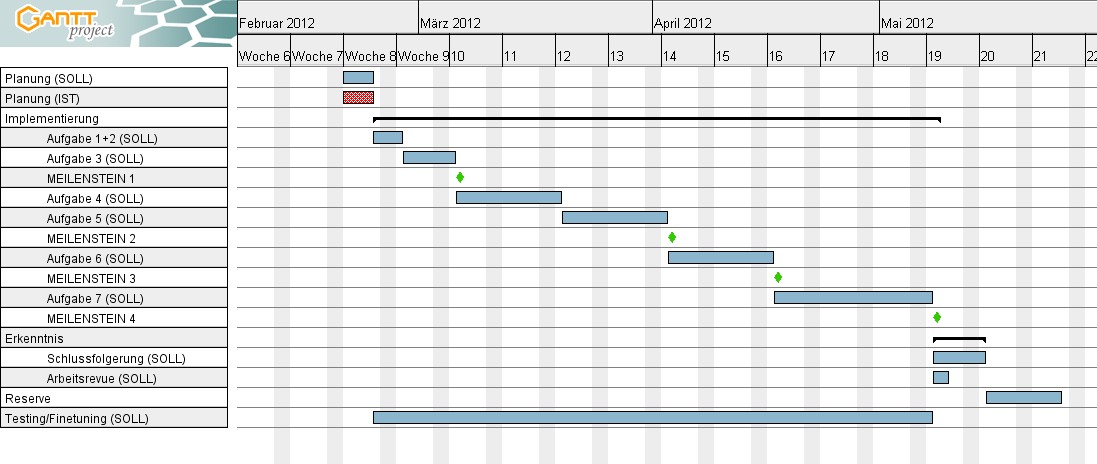
\includegraphics[width=1\linewidth]{img/projektplanung.png}
\caption{Projektplan}
\label{prplan}
\end{figure}

\subsection{Arbeitspakete}

\newpage

\part{Arbeitsberichte}
\newcommand\pgfmathsinandcos[3]{%
  \pgfmathsetmacro#1{sin(#3)}%
  \pgfmathsetmacro#2{cos(#3)}%
}

\newcommand\LongitudePlane[3][current plane]{%
  \pgfmathsinandcos\sinEl\cosEl{#2} % elevation
  \pgfmathsinandcos\sint\cost{#3} % azimuth
  \tikzset{#1/.estyle={cm={\cost,\sint*\sinEl,0,\cosEl,(0,0)}}}
}

\newcommand\LatitudePlane[3][current plane]{%
  \pgfmathsinandcos\sinEl\cosEl{#2} % elevation
  \pgfmathsinandcos\sint\cost{#3} % latitude
  \pgfmathsetmacro\yshift{\cosEl*\sint}
  \tikzset{#1/.estyle={cm={\cost,0,0,\cost*\sinEl,(0,\yshift)}}} %
}

\newcommand\DrawLongitudeCircle[2][1]{
  \LongitudePlane{\angEl}{#2}
  \tikzset{current plane/.prefix style={scale=#1}}
   % angle of "visibility"
  \pgfmathsetmacro\angVis{atan(sin(#2)*cos(\angEl)/sin(\angEl))} %
  \draw[current plane,thin,black] (\angVis:1) arc (\angVis:\angVis+180:1);
  \draw[current plane,thin,dashed] (\angVis-180:1) arc (\angVis-180:\angVis:1);
}%this is fake: for drawing the grid


\newcommand\DrawLongitudeCirclered[2][1]{
  \LongitudePlane{\angEl}{#2}
  \tikzset{current plane/.prefix style={scale=#1}}
   % angle of "visibility"
  \pgfmathsetmacro\angVis{atan(sin(#2)*cos(\angEl)/sin(\angEl))} %
  \draw[current plane,red,thick] (150:1) arc (150:180:1);
  %\draw[current plane,dashed] (-50:1) arc (-50:-35:1);
}%for drawing the grid


\newcommand\DLongredd[2][1]{
  \LongitudePlane{\angEl}{#2}
  \tikzset{current plane/.prefix style={scale=#1}}
   % angle of "visibility"
  \pgfmathsetmacro\angVis{atan(sin(#2)*cos(\angEl)/sin(\angEl))} %
  \draw[current plane,black,dashed, ultra thick] (150:1) arc (150:180:1);
}


\newcommand\DLatred[2][1]{
  \LatitudePlane{\angEl}{#2}
  \tikzset{current plane/.prefix style={scale=#1}}
  \pgfmathsetmacro\sinVis{sin(#2)/cos(#2)*sin(\angEl)/cos(\angEl)}
  % angle of "visibility"
  \pgfmathsetmacro\angVis{asin(min(1,max(\sinVis,-1)))}
  \draw[current plane,dashed,black,ultra thick] (-50:1) arc (-50:-35:1);
}


\newcommand\fillred[2][1]{
  \LongitudePlane{\angEl}{#2}
  \tikzset{current plane/.prefix style={scale=#1}}
   % angle of "visibility"
  \pgfmathsetmacro\angVis{atan(sin(#2)*cos(\angEl)/sin(\angEl))} %
  \draw[current plane,red,thin] (\angVis:1) arc (\angVis:\angVis+180:1);
}

\newcommand\DrawLatitudeCircle[2][1]{
  \LatitudePlane{\angEl}{#2}
  \tikzset{current plane/.prefix style={scale=#1}}
  \pgfmathsetmacro\sinVis{sin(#2)/cos(#2)*sin(\angEl)/cos(\angEl)}
  % angle of "visibility"
  \pgfmathsetmacro\angVis{asin(min(1,max(\sinVis,-1)))}
  \draw[current plane,thin,black] (\angVis:1) arc (\angVis:-\angVis-180:1);
  \draw[current plane,thin,dashed] (180-\angVis:1) arc (180-\angVis:\angVis:1);
}%Defining functions to draw limited latitude circles (for the red mesh)


\newcommand\DrawLatitudeCirclered[2][1]{
  \LatitudePlane{\angEl}{#2}
  \tikzset{current plane/.prefix style={scale=#1}}
  \pgfmathsetmacro\sinVis{sin(#2)/cos(#2)*sin(\angEl)/cos(\angEl)}
  % angle of "visibility"
  \pgfmathsetmacro\angVis{asin(min(1,max(\sinVis,-1)))}
  %\draw[current plane,red,thick] (-\angVis-50:1) arc (-\angVis-50:-\angVis-20:1);
\draw[current plane,red,thick] (-50:1) arc (-50:-35:1);
}


\tikzset{
  >=latex,
  inner sep=0pt,
  outer sep=2pt,
  mark coordinate/.style={inner sep=0pt,outer sep=0pt,minimum size=3pt, fill=black,circle}
}


\section{Aufgabe 1 - Orthodromie}
\subsection{Aufgabenstellung}
\begin{itemize}
  \item Erstellung eines Entscheidungsnetzes auf der Erdkugel
  \item Berechnung einer Orthodromie (Distanz in Meilen zwischen zwei Punkten auf der Erdkugel)
  \item Erstellung der Koordinatendatei eines Sees (in Koordinaten)
\end{itemize}

\subsection{Analyse der Problemstellung}
Auf einer Kugel soll zwischen zwei Punkten die kürzeste Route bzw. die kürzeste Verbindung gewählt werden. Dies wird durch das Vektorprodukt der beiden Vektoren vom Kugelursprung zu den beiden Punkten $A$ und $B$ einfach berechnet:

\begin{tikzpicture}[scale=1,every node/.style={minimum size=1cm}]
	%% some definitions
	
	\def\R{4} % sphere radius
	
	\def\angEl{25} % elevation angle
	\def\angAz{-100} % azimuth angle
	\def\angPhiOne{-50} % longitude of point P
	\def\angPhiTwo{-15} % longitude of point Q
	\def\angBeta{30} % latitude of point P and Q
	
	%% working planes
	
	\pgfmathsetmacro\H{\R*cos(\angEl)} % distance to north pole
	\LongitudePlane[xzplane]{\angEl}{\angAz}
	\LongitudePlane[pzplane]{\angEl}{\angPhiOne}
	\LongitudePlane[qzplane]{\angEl}{\angPhiTwo}
	\LatitudePlane[equator]{\angEl}{0}
	\fill[ball color=white!10] (0,0) circle (\R); % 3D lighting effect
	\coordinate (O) at (0,0);
	\coordinate[mark coordinate] (N) at (0,\H);
	\coordinate[mark coordinate] (S) at (0,-\H);
	
    \DrawLongitudeCircle[\R]{\angPhiOne} % pzplane
    \DrawLongitudeCircle[\R]{\angPhiTwo} % qzplane
    \DrawLatitudeCircle[\R]{\angBeta}
    \DrawLatitudeCircle[\R]{0} % equator
	%labelling north and south
	\node[above=8pt] at (N) {$\mathbf{N}$};
	\node[below=8pt] at (S) {$\mathbf{S}$};
        \draw[-,dashed, thick] (N) -- (S);	
    	
\end{tikzpicture}


\bibliographystyle{ba_zhaw}
\bibliography{hablumat_biblio,yuksefev_biblio}
 \end{document}
